\documentclass[a4paper, 12pt]{report}

% Поддержка русского языка
\usepackage[english, russian]{babel}
\usepackage[T2A]{fontenc}
\usepackage[utf8]{inputenc}
\usepackage{indentfirst}
\usepackage{hyperref}

\usepackage{amsmath, amsfonts, amssymb, amsthm, mathtools}

%% Оформление страницы
\usepackage{extsizes}     % Возможность сделать 14-й шрифт
\usepackage{geometry}     % Простой способ задавать поля
\usepackage{setspace}     % Интерлиньяж
\usepackage{enumitem}     % Настройка окружений itemize и enumerate
\setlist{leftmargin=25pt} % Отступы в itemize и enumerate

\geometry{top=25mm}    % Поля сверху страницы
\geometry{bottom=30mm} % Поля снизу страницы
\geometry{left=20mm}   % Поля слева страницы
\geometry{right=20mm}  % Поля справа страницы

\setlength\parindent{15pt}        % Устанавливает длину красной строки 15pt
\linespread{1.3}                  % Коэффициент межстрочного интервала
%\setlength{\parskip}{0.5em}      % Вертикальный интервал между абзацами
%\setcounter{secnumdepth}{0}      % Отключение нумерации разделов
%\setcounter{section}{-1}         % Нумерация секций с нуля
\usepackage{multicol}			  % Для текста в нескольких колонках
\usepackage{soulutf8}             % Модификаторы начертания

\newcommand{\nc}{\newcommand}

\nc{\Group}{\textbf{М8О-101Б-22}}
\nc{\Name}{\textbf{Кабанов Антон Алексеевич}}
\nc{\StudentNumber}{\textbf{7}}

\nc{\email}{\href{mailto:anton1258kab@gmail.com}{\textbf{anton1258kab@gmail.com}}}
\nc{\Contacts}{\email}

\nc{\Lecturer}{каф. 806 Крылов Сергей Сергеевич}

\nc{\Processor}{\textbf{AMD Ryzen 5500U (6-ядерный, @2.1 ГГц})}
\nc{\RAM}{\textbf{15345 Мб}}
\nc{\ROM}{\textbf{479.9 Гб}}
\nc{\Screen}{\textbf{встроенный, IPS, 2160x1440, @60 Гц}}

\nc{\OSFamily}{\textbf{GNU/Linux}}
\nc{\OSName}{\textbf{Manjaro Linux}}
\nc{\OSVersion}{\textbf{5.15.76-1-MANJARO}}
\nc{\Shell}{\textbf{bash}}
\nc{\ShellVersion}{\textbf{5.1.16}}

\nc{\ProgrammingLanguage}{\textbf{C}}
\nc{\TextEditor}{\textbf{emacs, vim (neovim)}}
\nc{\OSUtilities}{\textbf{pwd, who, ls, cd, mv, cp, rm, rmdir, mkdir, cat, whoami, man}}
\nc{\AppliedSystems}{\textbf{touch, echo, pacman, chmod, date, lsblk, gnuplot, emacs, nvim}}
\nc{\FileLocation}{\textbf{/home/void/Документы/FI-labs}}

\nc{\Equipment}{
	\textit{Оборудование ПЭВМ студента, если использовалось:} \\
	Процессор \Processor \ с ОП \RAM, ТТН \ROM. Монитор \Screen.
}

\nc{\Software}{
	\textit{Программное обеспечение ЭВМ студента, если использовалось:} \\
	Операционная система семейства \OSFamily, наименование \OSName \ версия \OSVersion, интерпретатор
	команд \Shell \ версия \ShellVersion. \\
	Система программирования: \ProgrammingLanguage \\
	Редактор текстов: \TextEditor \\
	Утилиты операционной системы: \OSUtilities \\
	Прикладные системы и программы: \AppliedSystems \\
	Местонахождение и имена файлов программ и данных на домашнем компьютере: \FileLocation
}

\usepackage{titleps}
\newpagestyle{main}{
	\setheadrule{0.1pt}
	\sethead{\DocName \ \Number}{}{}
	\setfootrule{0.1pt}
	\setfoot{}{}{\thepage}
}

\usepackage{xcolor}
\usepackage{listings}
\lstset{basicstyle=\ttfamily,
	showstringspaces=false,
	commentstyle=\color{red},
	keywordstyle=\color{blue}
}

\nc{\DocName}{Отчет по лабораторной работе}
\nc{\Number}{№ 6}
\nc{\CourseName}{Фундаментальная информатика}
\nc{\CompletionDate}{"18" октября 2022 г.}
\nc{\ReportDate}{"18" октября 2022 г.}
\nc{\Mark}{}
\nc{\Signature}{}
\nc{\Theme}{Конструирование диаграмм Тьюринга} %1
\nc{\Target}{Разработать диаграмму Тьюринга решения задачи в среде интерпретатора VTM или VisualTuring 2.0 с использованием стандартных машин ($r, l, R, L, K_n, i_a$) и вспомогательных машин, определяемых поставленной задачей. Вариант задания даётся преподавателем согласно выбранному студентом уровню сложности.} %2
\nc{\Task}{Перевод числа из шестнадцатиричной системы счисления в четверичную (линейная сложность)} %3
\nc{\Idea}{Два разряда числа в четверичной системе счисления эквивалентны по значению одному в шестнадцатеричной. Воспользуемся этим и будем постепенно отнимать у текущего разряда предварительно скопированного числа по единице и прибавлять ее к переводимому числу.} %6
\nc{\Plan}{} %7
\nc{\Protocol}{
	\\
	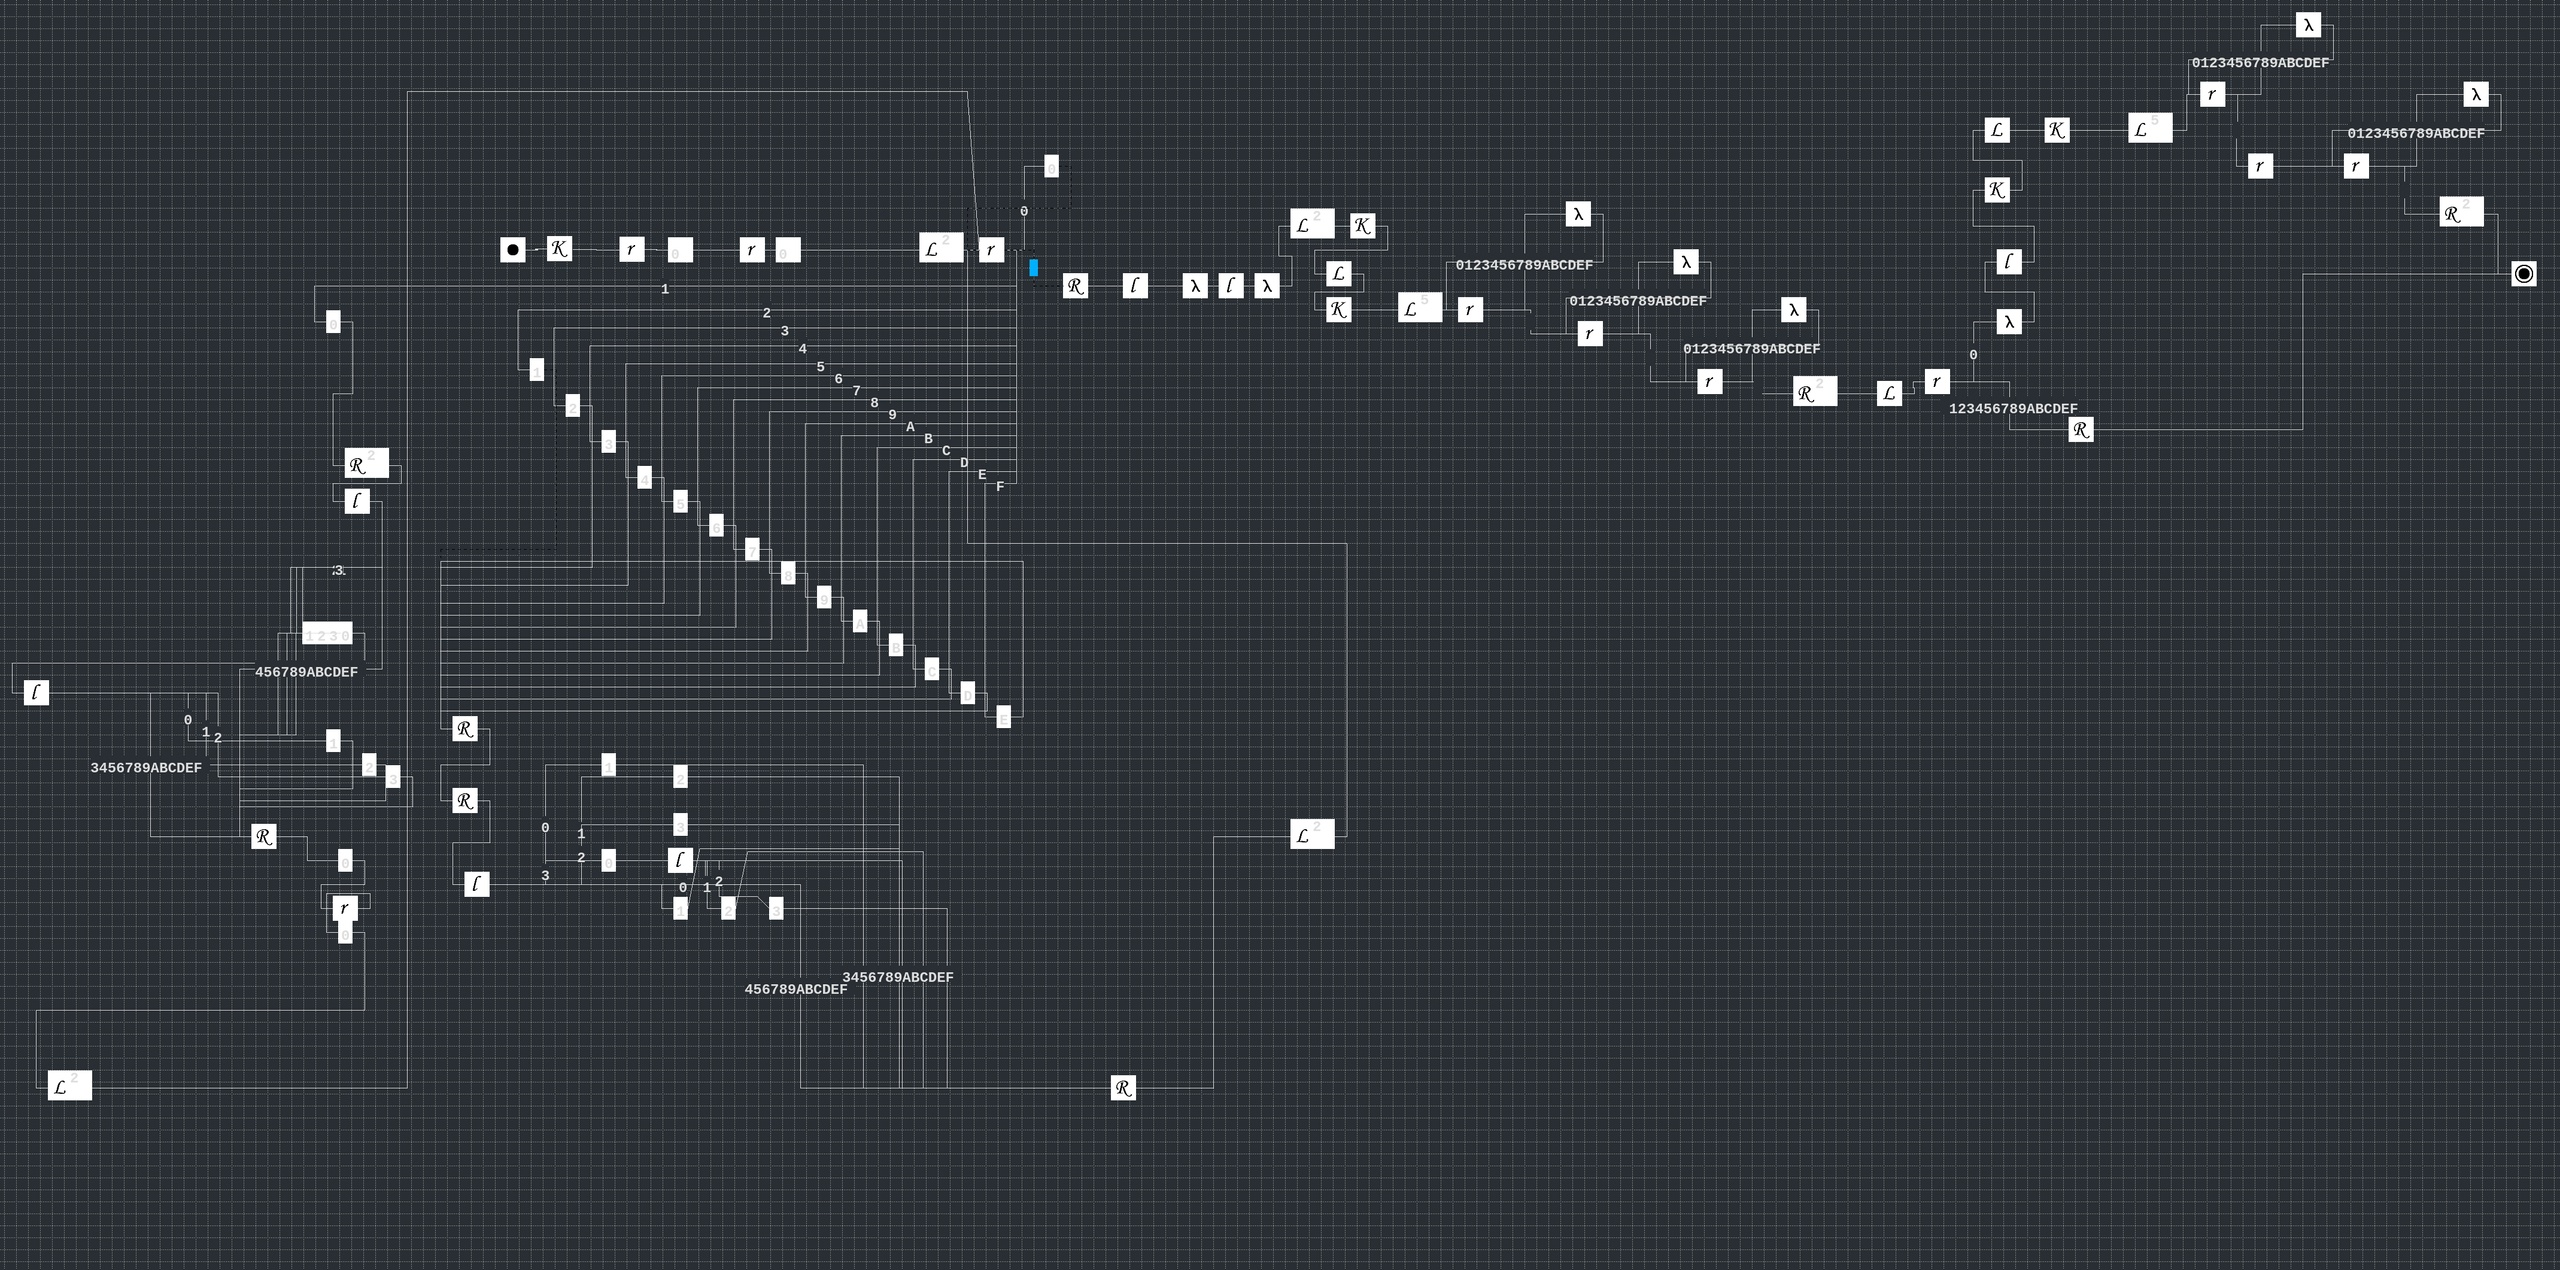
\includegraphics[width=\textwidth]{dmt.jpg}
	%без кириллицы:%
	%\lstinputlisting[caption={}, label={lst:listing-mt}, language=C]{l9.c}%
} %8
\nc{\Debugging}{
	\begin{tabular}{|c|c|c|c|p{3cm}|p{4cm}|l|}
		\hline
		№ & лаб/дом & Дата & Время & Событие & Действие по исправлению & Примечание \\
		\hline 
		& & & & & & \\
		\hline
	\end{tabular}
} %9
\nc{\AuthorRemarks}{-}
\nc{\Conclusions}{Я научился конструировать диаграммы Тьюринга.} %11
\nc{\Defects}{-}

\begin{document}
	\pagestyle{main}
\begin{large}
	\textbf{\DocName \ \Number \ по курсу \CourseName}
\end{large}	
\\
Студент группы: \Group, \ \Name, № по списку: \StudentNumber, контакты: \Contacts
\begin{flushright}
	Работа выполнена: \CompletionDate \\
	Преподаватель: \Lecturer \\
	Входной контроль знаний с оценкой: \\
	Отчет сдан \ReportDate, итоговая оценка \Mark \\
	Подпись преподавателя: \Signature
\end{flushright}
\begin{enumerate}
	\item \textbf{Тема:} \ \Theme
	\item \textbf{Цель работы: } \Target
	\item \textbf{Задание} \textit{(вариант № \StudentNumber)}: \Task
	\item \textbf{Оборудование:} \\ \Equipment
	\item \textbf{Программное обеспечение (лабораторное):} \\ \Software
	\item \textbf{Идея, метод, алгоритм} 
	\begin{footnotesize}
		решения задачи (в формах: словесной, псевдокода, графической [блок-схема, диаграмма, рисунок, таблица] или формальные спецификации с пред- и постусловиями)
	\end{footnotesize} 
	\\ \Idea
	\item \textbf{Сценарий выполнения работы}
	\begin{footnotesize}
		[план работы, первоначальный текст программы в черновике (можно на отдельном листе) и тесты либо соображения по тестированию]
	\end{footnotesize}
	\Plan
	\textit{Пункты 1-7 отчета составляются строго до начала лабораторной работы.}
	\begin{flushright}
		\textit{Допущен к выполнению работы.} \textbf{Подпись преподавателя:} 
	\end{flushright}
	\item \textbf{Распечатка протокола}
	\begin{footnotesize}
		(подклеить листинг окончательного варианта программы с тестовыми примерами, подписанный
		преподавателем):
	\end{footnotesize}
	\Protocol
	\item \textbf{Дневник отладки} 
	\begin{footnotesize}
		должен содержать дату и время сеансов отладки и основные события (ошибки в сценарии и программе,
		нестандартные ситуации) и краткие комментарии к ним. В дневнике отладки приводятся сведения об использовании других ЭВМ,
		существенном участии преподавателя и других лиц в написании и отладке программы:
	\end{footnotesize}
	\\
	\Debugging
	\item \textbf{Замечания автора} по существу работы: \AuthorsRemarks
	\item \textbf{Выводы:} \Conclusions
	\\
	Недочёты при выполнении задания могут быть устранены следующим образом: \Defects
	\begin{flushright}
		Подпись студента:
	\end{flushright}
\end{enumerate}
\end{document}
